\subsection{Architecture}
The actual architecture of the \ac{SDS} describes the structure of the \ac{SDS}. The elaboration models the architecture according to Starke's four-view principle. The four perspectives describe different aspects of the system architecture. \cite{starke_effektive_2020}

\subsubsection{Context perspective}\label{context_view}
The context perspective is an overview of the system by modeling out the dependencies to other systems and actors interacting with the system.\\
\begin{figure}[htbp]
    \centerline{
    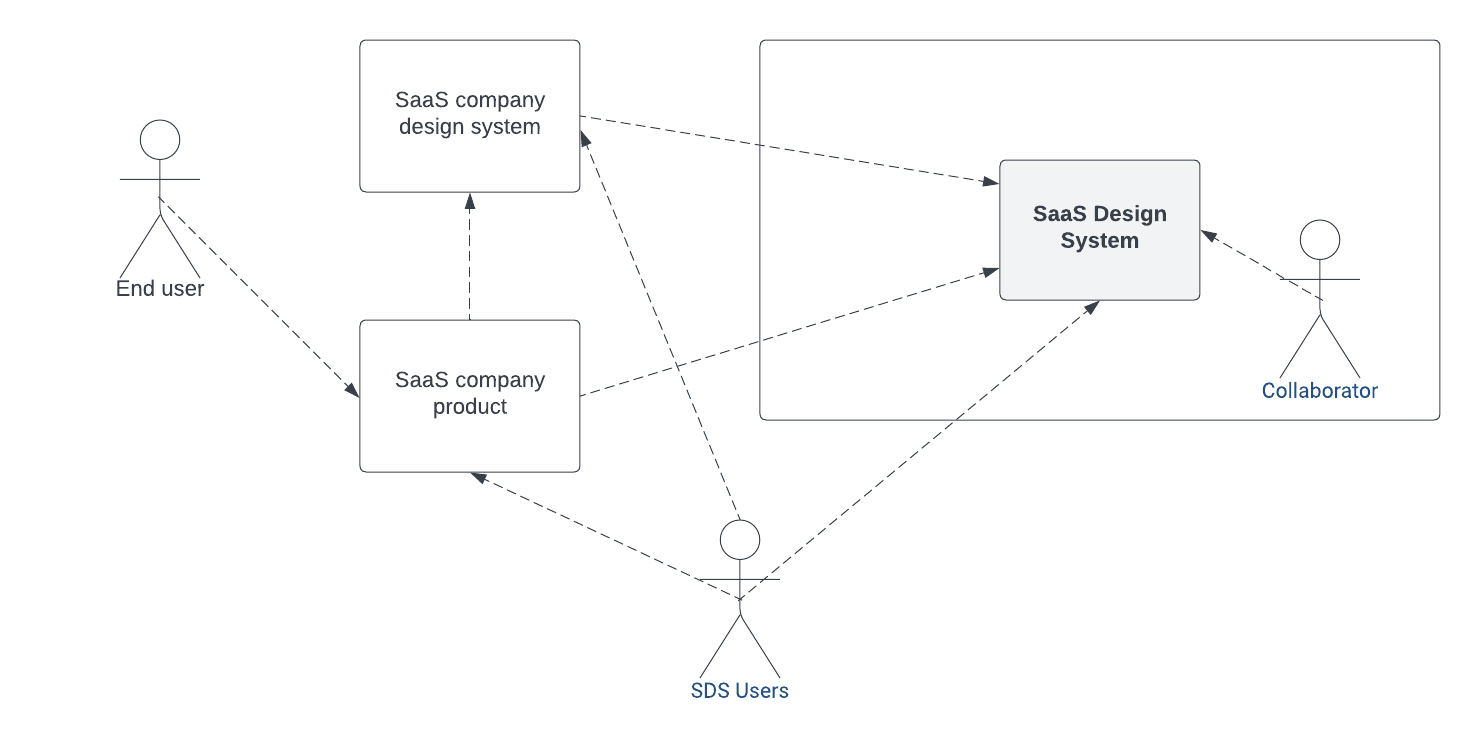
\includegraphics[width=\linewidth]{images/context_view_sds.png}}
\caption{Context perspective of \ac{SaaS} Design System}
\label{context_view_sds}
\end{figure}

Figure \ref{context_view_sds} shows the first view of \citeauthor{starke_effektive_2020}'s approach to modeling the system architecture - the context perspective. As described in the use case in Section \ref{sds_requirements}, the \ac{SDS} has three stakeholders interacting with the design system. The diagram shows the actively interacting stakeholders (\ac{SDS} users and collaborators) through their connections to the \ac{SDS}. \\
It also shows the "end user" who is not directly connected to the \ac{SDS}, but to a product from a \ac{SaaS} company. Nevertheless, it is important to mention the end user is the reason why the \ac{SDS} ultimately exists. Following the arrow trail that starts from the \ac{SaaS} company's product, the \ac{SDS} will always be the one to end up with. This means that the product uses the \ac{SDS} in some way either directly or through the company's design system. \\
The stakeholder who interacts directly with both the SDS and the company's product is the SDS user. User is perhaps a bit misleading, but if you take it that way, this persona uses the SDS to develop or design products from it. This stakeholder may also build the company's design system based on the SDS. This design system is then used by the company's products.\\
The last persona is the collaborator. The collaborator is not interested in applications or design systems that use SDS. The only thing the collaborator wants to do is contribute to the open source project. This is also the reason why this actor is placed inside the system, as the box around him represents the community around SDS.

\subsubsection{Building block view}
The building block view takes the architecture to the next level of detail. The diagrams use the context perspective and go all the way into the presented system, in this case \ac{SDS}. The view lists connections and dependencies to various things like frameworks, databases, components, scripts, and more. \\
The building block view consists of different layers. This makes it possible to focus on important aspects of the architecture in several steps. Diagrams abstract objects so that they can be discussed in more detail later. \cite{starke_effektive_2020} \\

\paragraph{Building block view level 1}
The only gray field in the context view (Figure \ref{context_view_sds}) is the \acl{SDS}. Therefore, the first view shows the top-level architecture of the design system. \\
\begin{figure}[htbp]
    \centerline{
    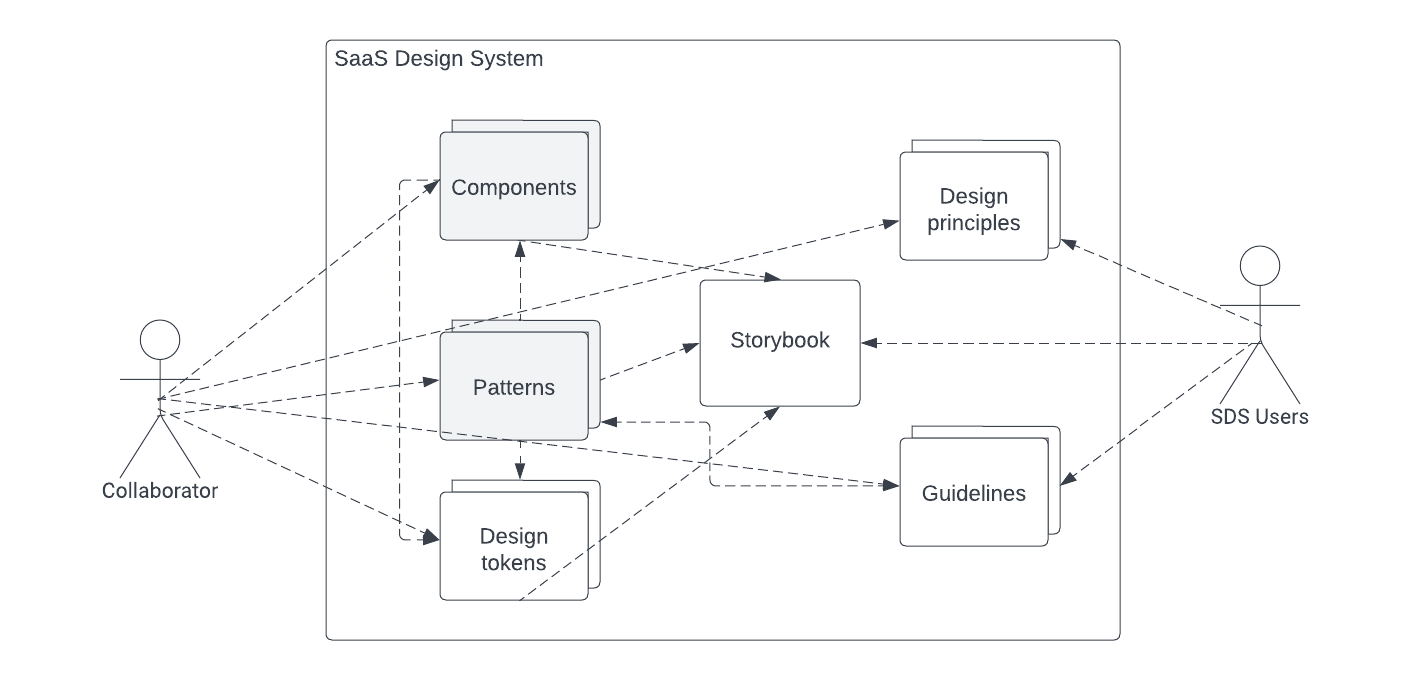
\includegraphics[width=\linewidth]{images/building_block_view_level_1.png}}
\caption{Building block view \ac{SDS} - level 1}
\label{building_block_level_1_sds}
\end{figure}
The level 1 building block view visible in Figure \ref{building_block_level_1_sds} consists of five elements and the two actors interacting with the design system in the context view. Since the SDS is a design system, most of the elements have already been explained in Chapter \ref{design_systems}.\\

\subparagraph{Storybook}
Storybook is the only component that is unknown. Storybook is a tool that helps create and document components on the web. Storybook makes it easy to develop components and document them at the same time. With a variety of plugins written by the community, it offers many possibilities to act as a documentation tool in a design system. \cite{storybook_storybook_nodate}\\
The diagram intentionally shows the building block in the middle. It serves as the central documentation system for components, patterns and design tokens. Therefore, the SDS user interacts with the storybook building block by searching for appropriate components for their use case. The diagram shows other relationships to the programmed assets of the design system. These connections represent the documentation aspect of these building blocks within Storybook.\\

\subparagraph{Design principles}
Design principles are another building block of \ac{SDS}. The diagram in Figure \ref{building_block_level_1_sds} shows that this building block has connections to collaborators and the \ac{SDS} user. This is because both actors use design principles when interacting with the \ac{SDS}. The \ac{SDS} user should keep these principles in mind when creating new applications with the \ac{SDS} or extending the \ac{SDS} to create their own design system. On the other hand, the collaborator keeps the principles in mind when contributing to the system. Components, patterns, and tokens should always follow the design principles. \\
In terms of design principles, the \ac{SDS} strives to keep them lean and easy to understand. This helps the design system to serve as a basis for other design systems. \\
The \textbf{Simple} principle states that component design should not have unnecessary styles or features that make it difficult to extend. This principle underlines the idea of keeping the entire design system lean. Developers understand lean descriptions and clear documentation much better than reading a wall of text. \\
Many products strive to implement accessibility in their products. With the \textbf{Accessible} principle, \ac{SDS} emphasizes the importance of accessible user interfaces. This emphasizes not only significant in terms of inclusion, but also helps accessibility in the overall user experience for all users. Because \textbf{Accessibility} doesn't just come into play when it relates to disabilities, it helps the application with the overall user experience. \\
The third and final principle is \textbf{Solid}. As stated earlier, the \ac{SDS} is a foundation for other design systems to build upon. Therefore, the importance of a stable and consistent API is paramount. Components and patterns should not change regularly. Versioning allows developers to choose their desired version of the \ac{SDS} without having to adapt. For this reason, the design system has deliberately chosen \textbf{Solid} as the third and final principle. \\
The first iteration of the \acl{SDS} principles provides a good foundation on which to build. As described in Chapter \ref{design_principles}, finding the right design principles will take a few iterations to get right. But by starting with \textbf{Simple}, \textbf{Accessible}, and \textbf{Solid}, designers and developers will find the right way to use this design system.

\subparagraph{Guidelines}
The next building block that the SDS user comes into contact with are guidelines. It is obvious that the SDS user needs to know about guidelines in a design system, hence the connection. Furthermore, the diagram shows a bidirectional connection to patterns, which is interpreted as a close cooperation between guidelines and patterns in \ac{SDS}.\\
The design principles just presented form the basis for the \ac{SDS} guidelines. In addition to the core extension, accessibility, and basic use guidelines, some guidelines focus on contributions and collaboration. Therefore, the diagram adds a link to collaborators to the guidelines. This emphasizes that collaborators also consume the guidelines of the design system. As this is an open-source system, as many people as possible should be able to work on it. \\
The extension guidelines address how to integrate \ac{SDS} as the basis for a company's own design system. It shows developers and designers how to create their own from the components provided. The goal of such a guide is to help system developers use the SDS as a foundation. The guide helps developers and designers to build their system on the SDS instead of introducing complex integrations. \\
Since accessibility is also a design principle, a guideline must define what the \ac{SDS} means by accessibility. The guideline should give the user a definition and sources for accessibility. But there should also be a manual for self-designed components to help users implement accessibility. Understanding this guide, users should no longer have accessibility questions when designing new interfaces. \\
As a third guideline, the \ac{SDS} will support the user in using the system. This guide could also be seen as an entry guide and will cover the basics. Importing the design system, proper bootstrapping, and guidance on configuring the system. Such a guideline may seem self-explanatory, but the lack of it often prevents users from using the system. The usage guide should be as simple as possible and cover every small step needed to get started with the \ac{SDS}. \\
One goal of this design system is to be developed by the community for the community. However, this can quickly get out of hand if everyone contributes without guidance. Therefore, it is crucial to introduce some from the beginning. This guide guides how to contribute to the component library and enforce changes to the guidelines and principles. \\
As this design system evolves over time, there should be opportunities to change and adapt. What this will look like in the end will evolve over time. What this will look like in the end will evolve. Some ideas could be a voting process or an RFC process, as is standard in the software industry. \\
Some design systems introduce blogs and forums for knowledge exchange to achieve high interactivity in a design system. In this way, users can connect, discuss and contribute to ideas to further improve the design system. A well-moderated blog and forum will further enhance the community around the \ac{SDS}. \\
Since the \ac{SDS} won't be a product but an open source project, forums and blogs will be the marketing platform to spread the idea of the design system. The goal is to build a strong community around the \ac{SDS}. So that some of the advocates end up contributing to the actual design system. \\
In summary, the guidelines of the \acl{SDS} are about creating a community around the design system. Developer and designers should not only using it for their desired goal, but see the potential to collaborate for the bigger picture behind \ac{SDS}.

\subparagraph{Design tokens}
The last non-gray box in the diagram in Figure \ref{building_block_level_1_sds} is the building block of design tokens. Design tokens form the basis for each component or pattern. Tokens are the smallest unit within the \ac{SDS}. Yet, design tokens have many connections to other building blocks within the design system. 
The connection to collaborators represents their contributions to the design tokens. Collaborators maintain the design tokens. The other two incoming links to components and patterns represent the use of design tokens in them. As well as the link to Storybook described earlier to document Design Tokens for \ac{SDS} users.
\ac{SDS}'s design tokens are not very specific. They consist of basic values like colors, spacing, typography, which were also described in Chapter \ref{layout}.\\

Next, it is time to take a closer look at the architecture of the SDS by moving to the second level of the building block view. At the second level, Starke's method performs a more detailed analysis of the building blocks of the components and patterns.

\paragraph{Building block view level 2 - Components}
The first detailed view deals with the components of SDS. Figure \ref{building_block_level_2_component_sds} shows the diagram of a second level component block view. The component building block is in the middle of this diagram. A lot of connections start from there.

\begin{figure}[htbp]
    \centerline{
    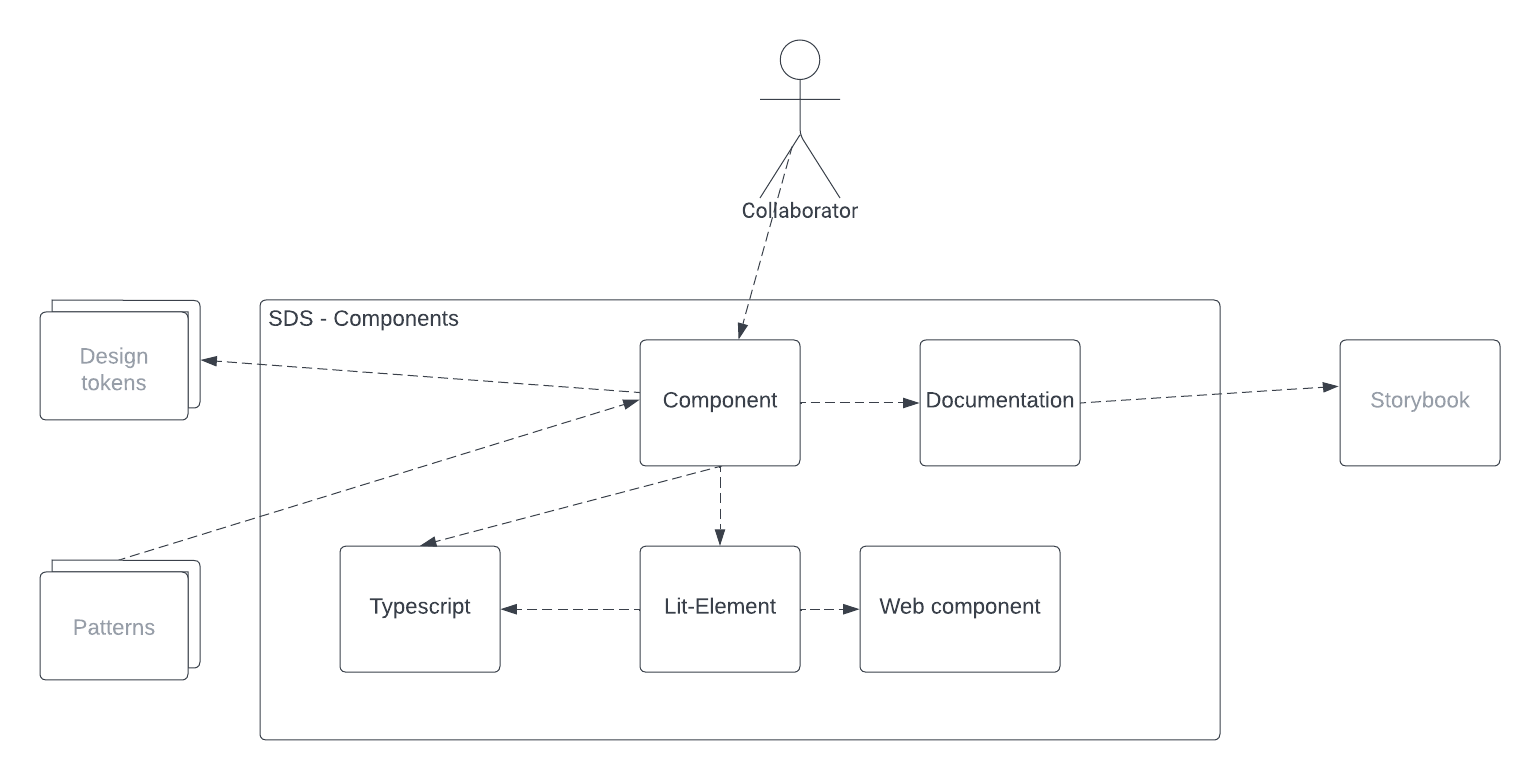
\includegraphics[width=\linewidth]{images/building_block_view_level_2_component.png}}
\caption{Building block level 2 component}
\label{building_block_level_2_component_sds}
\end{figure}
\subparagraph{Component} \label{sds-component}
Without well-assembled components, design systems cannot exist. Therefore, choosing the right technology package for building components is very important. In the case of \ac{SDS}, one of the most essential requirements is that the system is usable independently of the frontend framework used. The link to the Lit element module symbolizes the use of this lightweight framework, which can be used to create framework-independent components. In addition to this link, the link to Typescript points to another technology that supports building the components.  \\
The diagram shows that the only actor in the components of the design system is the collaborator. He is responsible for all adjustments of the component. \\
Since components within a design system must have documentation, this diagram shows a link from the component box to the documentation building block. This indicator shows that a component provides documentation that is then used further in the storybook component to publish it. \\
Other outgoing connections related to the component module are to the other essential components of a design system - the tokens and patterns. As explained earlier, tokens should be used everywhere when new elements are created within the design system. The connection represents the consumption of design tokens in a component. The other outgoing connection is actually a consumption of the components by the design system patterns. \\

\subparagraph{Typescript}
To further assist developers, \ac{SDS} uses Typescript, a superset of Javascript. It extends Javascript with types and interfaces. Typescript must be compiled into Javascript for the browser to understand, but this allows the developer to find errors much faster because it fails at compile time rather than at runtime. \citep{microsoft_typescript_nodate} \\
For this reason, the diagram in Figure \ref{building_block_level_2_component_sds} shows that Typescript is used by the Lit element and the component module. Therefore, technologically, there is no gap between the component and the framework used.

\subparagraph{Lit-Element}
Creating web components natively can be complicated. The Lit Element framework helps developers build web components by eliminating some of the pitfalls of implementing web components from scratch. With a focus on ease of understanding, intelligent \ac{DOM} updates, and a small package size (5 KB), Lit is a perfect addition for creating components for design systems based on standard web components. \citep{lit_nodate} \\
Since this framework is based on the web standard of web components, the diagram indicates the use of this standard with a link.

\subparagraph{Web components}
Web Components is a widely supported standard in all modern browsers for creating reusable components. It is not necessary to use a framework like React or Angular. Web Components encapsulate \ac{HTML}, \ac{CSS}, and JavaScript from the rest of the elements within a browser. They provide interfaces for communicating data in and out of the component. This makes web components highly reusable in all parts of a web project. \citep{mdn_web_component_nodate} \\
Due to their high reusability and broad support, web components are a perfect fit for \ac{SDS} components. As described in the previous section, the link in the diagram represents the use of the Web Components standard by Lit-Element.

\subparagraph{Documentation}
Last but not least, users must have access to the documentation of components. The link in Figure \ref{building_block_level_2_component_sds} from the documentation to the Storybook indicates that it is the documentation tool for the \ac{SDS}. \\
With MDX, the combination of Markdown templating (MD) and code injection via JSX, it is possible to write fluid documentation without having to jump back and forth between files while documenting components. \citep{otander_markdown_2017} \\

\paragraph{Building block view level 2 - Patterns}
The second detailed view deals with the patterns of SDS. Figure \ref{building_block_level_2_pattern_sds} shows the diagram of a second level component block view. The pattern building block is in the middle of this diagram. A lot of connections start from there.
\begin{figure}[htbp]
    \centerline{
    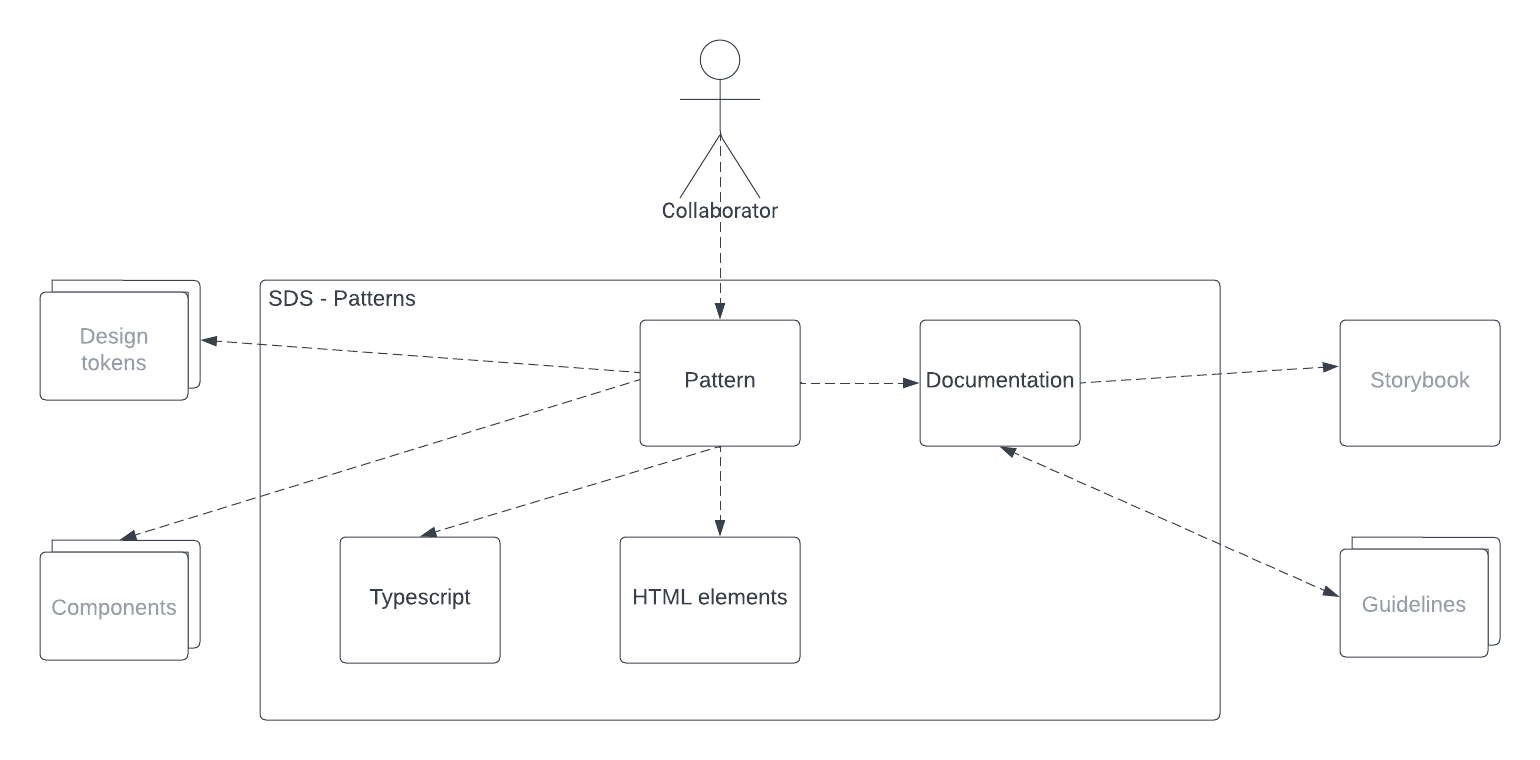
\includegraphics[width=\linewidth]{images/building_block_view_level_2_pattern.png}}
\caption{Building block level 2 pattern}
\label{building_block_level_2_pattern_sds}
\end{figure}



\subparagraph{Pattern}
An essential part of a design systems are patterns. Patterns try to combine the capabilities of a design system with the design of user interfaces. In the case of \ac{SDS}, patterns help developers automatically apply best practices to their product without having to read an entire text. \\
As with the components of SDS, the only actor is the collaborator. Figure \ref{building_block_level_2_pattern_sds} shows the only link of an actor to the pattern, indicating that he is responsible for all pattern adjustments. \\
Combining standard \ac{HTML} elements and components from SDS creates patterns in SDS. The diagram indicates these connections by the arrows shown above. These patterns are easily accessible to the developer by copying and pasting code into the desired application that integrates the \ac{SDS}. \\
Patterns use design tokens and components of \ac{SDS}, visible here in Figure \ref{building_block_level_2_pattern_sds} as external dependencies. This ensures that the patterns created are consistent with the overall design idea of the design system. \\
Additional documentation, visible through the connection with the documentation module, helps the developer to avoid using patterns where they do not belong. \\
The goal of \ac{SDS} patterns is to simplify web accessibility compliance and leave enough room for user customization. Proper use of patterns is crucial for successful integration of \ac{SDS} into a product.

\subparagraph{Documentation}
\ac{SDS} patterns come with special documentation that allows for customization and redesign. The documentation enables developers to fulfill their requirements for their own design system.\\
As with the component documentation, a link to the storybook shows that the patterns also leverage the power of the features. Features such as live examples show the \ac{SDS} user how the design system patterns will work in the final product. Several different examples for each pattern present the possibilities for individual design. \\
A special link in Figure \ref{building_block_level_2_pattern_sds} shows the bidirectional connection from documentation to guidelines. This link represents the possibility to share own variants of the \ac{SDS} design patterns. This leads to a high level of interaction of the design patterns within the \acl{SDS}.

\subparagraph{\ac{HTML} elements}
The last block in the diagram of Figure \ref{building_block_level_2_pattern_sds} is the \ac{HTML} element. This block is there for several reasons. It's not just about the use of \ac{HTML} elements within patterns, but also about their proper use. \\
\ac{HTML} elements have a lot of built-in accessibility, and that's what SDS's patterns are looking for. Proper use of \ac{HTML} elements helps structure the code of a web page while providing accessibility for keyboards and screen readers. \citep{mdn_html_nodate}

\subsubsection{Runtime view}
The runtime view is the third view of Starke's four-view principle. Here it is important to find out which components are active for a particular action. This helps to understand which components interact with each other and when, and which preconditions are required for certain processes. \citep{starke_effektive_2020}\\
An existing use case of a runtime diagram is the interaction of the end user with an application that implements the \ac{SDS}. Considering the context view in Chapter \ref{context_view}, the end user does not interact directly with the \ac{SDS}. Therefore, a sequence diagram helps to understand how the end user ultimately interacts with the \ac{SDS}. \\
\begin{figure}[htb]
    \centerline{
    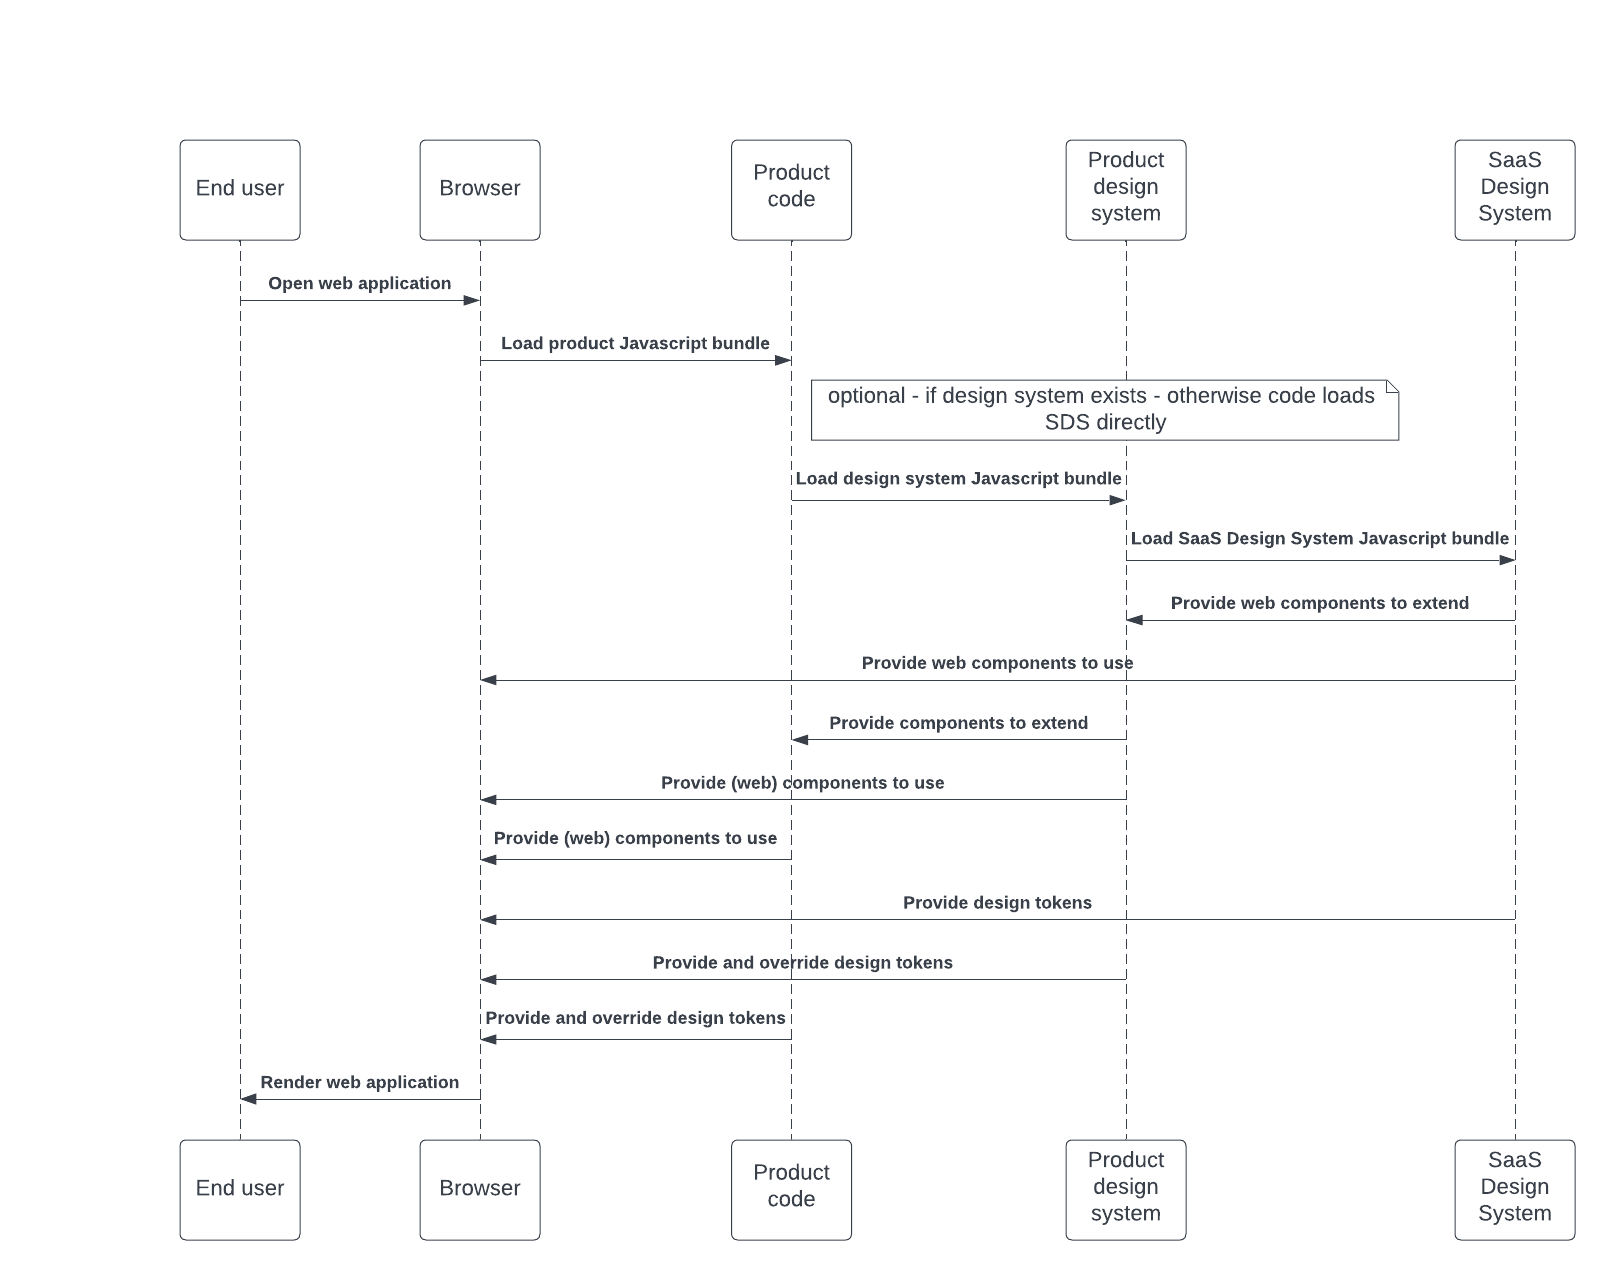
\includegraphics[width=\linewidth]{images/runtime_diagram_sds.png}}
\caption{Run time diagram of end user interacting with \ac{SDS}}
\label{runtime_diagram_sds}
\end{figure}
The following steps explain the flow of the sequence diagram shown in Figure \ref{runtime_diagram_sds}.
\begin{enumerate}
    \item The end user starts by opening the web browser and accessing a \ac{SaaS} web application. 
    \item The opened web application initiates a load of preferentially bundled JavaScript files from the \ac{SaaS} product.
    \item  Within the bundled code of the product, components of a component library from a product design system may be included. 
    \item The product design system is based on the \acl{SDS}, therefore the \ac{SDS} is loaded.
    \item In return, the \ac{SDS} provides the product development system with the component code as the basis for its components.
    \item The \ac{SDS} also makes the same components available to the browser so that they are available for rendering.
    \item The product design system returns its component to the product code.
    \item The product design system also makes its components available to the browser so that they are available for rendering.
    \item When all the component information is available, the product code can make the final changes to the components and then return them to the browser for rendering.
    \item The design tokens of the \ac{SDS} are provided in the root of the browser.
    \item The design tokens of the product design system are provided in the root of the browser. This will override the tokens of the \ac{SDS}.
    \item The product code has its own design tokens and overrides them in the last instance.
    \item After completing all the steps, the browser is able to render the desired web application for the end user.
\end{enumerate}
It is important to note in this diagram that the steps (10-12) to load the design tokens in the browser do not have to be behind the component code. Rather, the tokens can be loaded into the browser in parallel. It is only important to note the order in which the design tokens override each other. \\
As well as the note inside the diagram. It is not necessary to have a design system of a product team between the use of the \ac{SDS}. It is also possible for a \ac{SaaS} product to use the \ac{SDS} directly.\\
This completes the runtime view of the end user interacting with the SDS. 
\subsubsection{Distribution view}
The fourth and final view of Starke's model is the distribution view. The goal of this view is to show how the system distributes its components. This makes it possible to show crucial interfaces between system components. A distribution diagram displays how components are distributed across the system infrastructure. This view is especially important for the operators of the software system. \cite{starke_effektive_2020} \\
\begin{figure}[htbp]
    \centerline{
    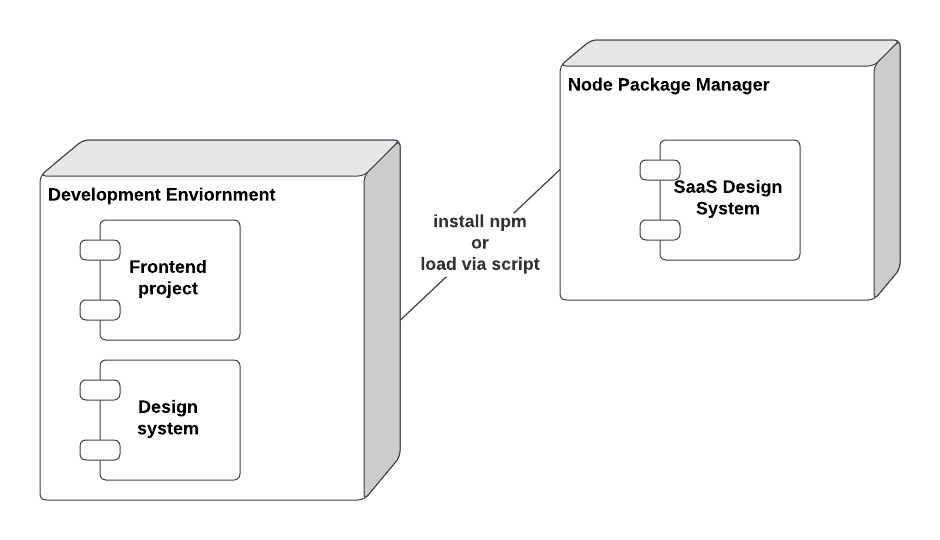
\includegraphics[width=\linewidth]{images/deployment_diagram_sds.png}}
\caption{Deployment diagram of \ac{SDS}}
\label{deployment_diagram_sds}
\end{figure}
In the case of SDS, a deployment view is difficult to model. Since the design system does not require a backend or database service. The only thing the SDS does is to deploy a bundled JavaScript file via a package manager. This way, the component library is available to everyone. \\
Figure \ref{deployment_diagram_sds} shows exactly this scenario. The developed design system is deployed in a package manager, in this case the Node package manager. On the left side of the diagram is the local development environment of each developer using the \ac{SDS}. As before, he could have a design system built on top of the \ac{SDS}. \\
In either case, this local development environment receives the design system through the channel shown in Figure \ref{deployment_diagram_sds}. This channel can either be loaded via a script tag within his web project or installed via the Node package manager within his environment.  